\documentclass[reprint, amsmath,amssymb,aps]{revtex4-2}
\usepackage{latex/project-preamble}
\usepackage{latex/project-macros}
\usepackage{latex/project-boxes}
\begin{document}
\title{Transport through a ferromagnet-bilayer-graphene-superconductor junction}
\author{A. I. González$^{1}$}
\author{P. A. Orellana$^{1}$}
\author{E. C. Siqueira$^{2}$}
\email{ecosta@utfpr.edu.br}
\affiliation{
	$^{1}$Departamento de Física, Universidad Técnica Federico Santa María, 110 V, Valparaíso, Casilla, Chile\\
	$^{2}$Departamento de Física, Universidade Tecnológica Federal do Paraná (UTFPR), 84016-210, Ponta Grossa, PR, Brasil}
\date{\today}
\maketitle

% ------------------------- TEXT OF THE MANUSCRIPT -------------------------

\section{\label{sec:model} Model and Formulation}
%In this section, we develop the model and formalism used to characterize the transport through the system.

%\subsection{Geometry and lattice convention}
The system is illustrated in Fig. \ref{figgeometry}. It is composed by two layers, labeled by $j=1,2$, coupled in two geometries referred as $1\rightarrow 1$ and $1\rightarrow 2$. These correspond to the Fig. \ref{figgeometry} (a) and Fig. \ref{figgeometry} (b), respectively. The transversal and longitudinal direction are indexed by $n$ and $m$ integers, respectively. Using this convention, we notice that the graphene-bilayer is located in the range $1\le m\le N$, for both geometries. For $m\leq 0$, the graphene monolayer is assumed to be ferromagnetic, while for $m\geq N+1$, there is the \textit{s-wave} superconductor monolayer. The main difference between both geometries regards the coupling between the grapahene-bilayer and the superconductor monolayer at its right side. In fact, for $1\rightarrow 1$ geometry, the superconductor is coupled to the lower monolayer while in the geometry $1\rightarrow 2$, the superconductor monolayer is coupled to the upper layer. This is more clearly visualized in Fig. \ref{figgeometry}(d), where a block diagram of the system is shown. We also point out that for both geometries we have assumed a Bernal stacking, as shown in Fig. \ref{figgeometry}(c), where an atom of $A$-atom of the lower monolayer is coupled to an $B$ atom of the upper monolayer.
\begin{figure*}[!]\centering
	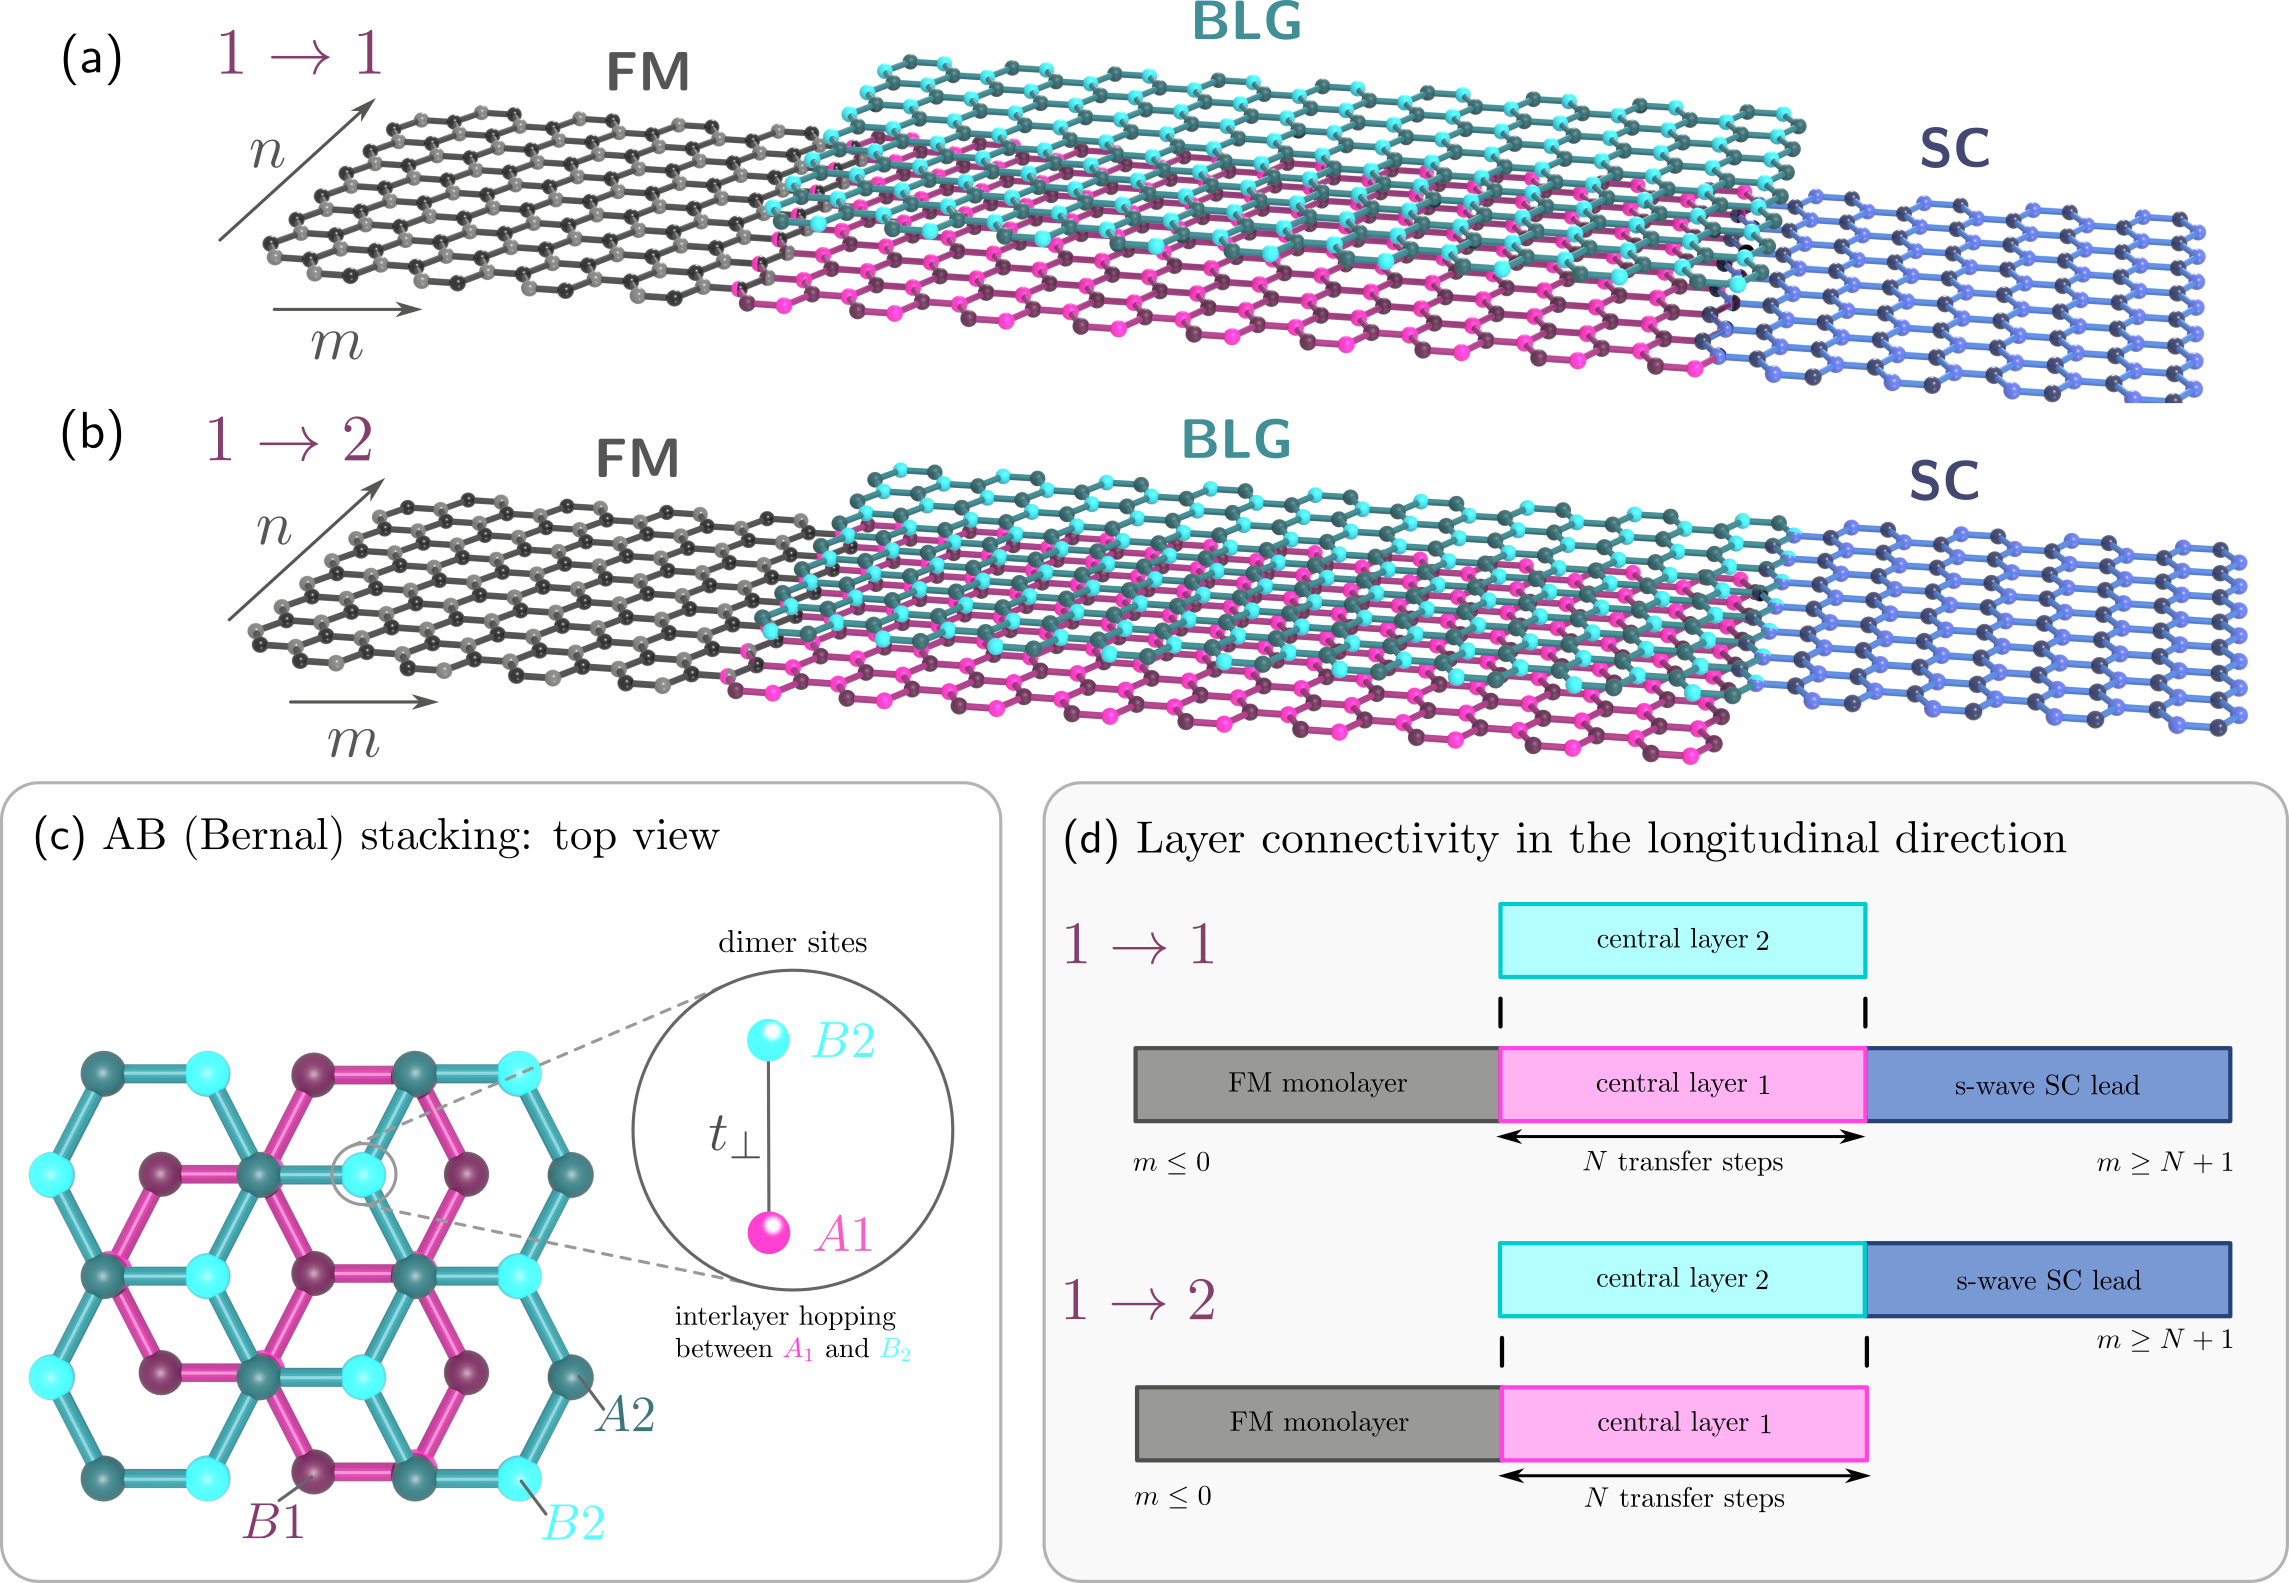
\includegraphics[scale=0.22]{figures/system.png}
	\caption{\label{figgeometry}
		Geometry, lattice structure, and longitudinal connectivity of the
		ferromagnet--bilayer-graphene--superconductor (FM--BLG--SC)
		junction.
		(a)~Atomic representation of the $1\!\to\!1$ geometry, in which
		the ferromagnetic (FM) and superconducting (SC) monolayer graphene
		leads are connected to the same layer of the finite bilayer graphene
		(BLG) region.
		(b)~Corresponding $1\!\to\!2$ geometry, in which the FM and SC
		leads are connected to opposite graphene layers.
		The longitudinal and transverse lattice directions are denoted by
		$m$ and $n$, respectively.
		Gray, magenta, cyan, and indigo identify the FM monolayer,
		central layer~1, central layer~2, and SC monolayer, respectively.
		(c)~Top view of the AB (Bernal) stacking in the central bilayer.
		Different shades within each layer distinguish the $A$ and $B$
		sublattices.
		The enlarged detail shows the vertically registered $A_1$ and
		$B_2$ dimer sites, coupled by the interlayer hopping $t_\perp$;
		the $A_1$ site is hidden beneath $B_2$ in the top projection.
		The non-dimer sites $B_1$ and $A_2$ are also indicated.
		(d)~Longitudinal layer-connectivity representation of the
		$1\!\to\!1$ and $1\!\to\!2$ junctions.
		The FM lead occupies $m\leq0$, the finite BLG region extends over
		$N$ transfer steps, $1\leq m\leq N$, and the SC lead occupies
		$m\geq N+1$.
		In the $1\!\to\!1$ geometry the SC lead continues from central
		layer~1, whereas in the $1\!\to\!2$ geometry it continues from
		central layer~2.%
	}
\end{figure*}

\subsection{The Model}



Next, we define the Hamiltonian for each section of the system illustrated in Fig. \ref{figgeometry}.
\subsubsection{Coupling Hamiltonian}
By assuming a nearest-neighbour approximation, each $A$ site is connected to three $B$ sites. As a result, the
intralayer Hamiltonian is
\begin{align}
	\hat H_{t}=-t\sum_{j,\sigma\atop{m,n}}
	\hat a_{jmn\sigma}^{\dagger}
	\left(
	\hat b_{jmn\sigma}+
	\hat b_{j,m+1,n,\sigma}+
	\hat b_{j,m,n+1,\sigma}
	\right)+\hc,
	\label{eq:H-t}
\end{align}
where we have also added the indexes $j=(1,2)$ that identifies the lower and upper monolayers, respectively, and the index $\sigma=(\uparrow,\downarrow)$, in order to identify the electron spin, since the ferromagnet polarization breaks the spin symmetry.


In order to account for the coupling between lower and upper monolayer, we define the Hamiltonian $\hat{H}_{\perp}$ whose form is given by:
\begin{equation}
	\hat H_\perp=-t_\perp
	\sum_{m=1}^{N}\sum_{n,\sigma}
	\left(
	\hat a_{1mn\sigma}^{\dagger}\hat b_{2mn\sigma}+\hc
	\right),
	\label{eq:H-perp}
\end{equation}
since we are using  AB stacking, the dimer bond connects $A_1$ to $B_2$.  Notice that it exists only in range $0\leq m\leq N$ where the bilayer is defined.

\subsubsection{Chemical potentials, gate potentials, and exchange field}
In order to take the different physical correlations at each section of the system, we define the on-site Hamiltonian as follows:
\begin{equation}
	\hat H_{\rm on}=\sum_{j,m,n,\alpha,\sigma}
	\left[V_j(m)-\mu(m)-s_\sigma h(m)\right]
	\hat n_{jmn\alpha\sigma},
	\label{eq:H-onsite}
\end{equation}
where we have defined the number operator,
\begin{equation}
	\hat n_{jmn\alpha\sigma}=
	\hat c_{jmn\alpha\sigma}^{\dagger}
	\hat c_{jmn\alpha\sigma}.
\end{equation}

In Eq. \eqref{eq:H-onsite}, $s_\uparrow=+1$, $s_\downarrow=-1$ and the additional index $\alpha$ identifies which monolayer section is being considered, i.e., ferromagnetic, central bilayer, and right superconductor monolayer. In this way, $\alpha = F, C, S$.

The chemical potential is piecewise constant,
\begin{equation}
	\mu(m)=
	\begin{cases}
		\mu_F, & m\le0,       \\
		\mu_C, & 1\le m\le N, \\
		\mu_S, & m\ge N+1,
	\end{cases}
\end{equation}
and the collinear exchange field is
\begin{equation}
	h(m)=
	\begin{cases}
		h, & m\le0, \\
		0, & m\ge1.
	\end{cases}
\end{equation}

The central layer potentials $V_1,V_2$ account for a gate bias applied to each monolayer.

\subsubsection{Onsite spin-singlet pairing}

The superconducting lead contains an onsite pair potential,
\begin{equation}
	\hat H_\Delta=\sum_{j,m,n,\alpha}
	\left[
		\Delta(m)\hat c_{jmn\alpha\uparrow}^{\dagger}
		\hat c_{jmn\alpha\downarrow}^{\dagger}
		+\Delta^*(m)\hat c_{jmn\alpha\downarrow}
		\hat c_{jmn\alpha\uparrow}
		\right],
	\label{eq:H-pair}
\end{equation}
with
\begin{equation}
	\Delta(m)=
	\begin{cases}
		0,                        & m\le N,   \\
		\Delta_0\ee^{\ii\varphi}, & m\ge N+1.
	\end{cases}
\end{equation}
Because pairing is onsite, it connects electron and hole amplitudes on the same
layer and sublattice.  There is no pairing during propagation through the
central bilayer.

\subsubsection{Complete Hamiltonian}

By combining Eqs. \eqref{eq:H-t}, \eqref{eq:H-perp}, \eqref{eq:H-onsite}, \eqref{eq:H-pair} we have the following complete Hamiltonian for the whole system that constitutes the miscroscopic model of the system illustrated in Fig. \ref{figgeometry}:
\begin{equation}
	\hat H=
	\hat H_t+\hat H_\perp+
	\hat H_{\rm on}+\hat H_\Delta.
	\label{eq:H-total}
\end{equation}

In Eq. \eqref{eq:H-total}, no interface barrier is added phenomenologically.  Contact mismatch arises
from the actual change in layer number, exchange field, chemical potential,
and pairing.

\subsection{Transverse Fourier transformation and Bogoliubov-de Gennes (BdG) equations}

We assume translational invariance along the transversal direction, in this way, we can perform a Fourier transformation along the $y$-direction. By assuming $N_y$ transverse cells with periodic boundary conditions, we write:
\begin{align*}
	\hat a_{jmn\sigma} & =\frac{1}{\sqrt{N_y}}
	\sum_K\ee^{\ii Kn}\hat a_{jmK\sigma},
	\\
	\hat b_{jmn\sigma} & =\frac{1}{\sqrt{N_y}}
	\sum_K\ee^{\ii Kn}\hat b_{jmK\sigma},
	\label{eq:FT}
\end{align*}
with $K$ being the transverse momentum. By substituting these expressions into Eq. \eqref{eq:H-total}, we obtain a set of independent equations. In particular, Eq. \eqref{eq:H-t} becomes:
\begin{equation}
	\hat H_t(K)=-\sum_{j,m,\sigma}
	\left[
		\eta\hat a_{jmK\sigma}^{\dagger}\hat b_{jmK\sigma}
		+\xi\hat a_{jmK\sigma}^{\dagger}\hat b_{j,m+1,K,\sigma}
		+\hc
		\right],
	\label{eq:H-t-K}
\end{equation}
with
\begin{equation}
	\eta(K)=t(1+\ee^{\ii K}),
	\qquad
	\xi=t,
	\label{eq:eta-xi}
\end{equation}
where the symbol $\eta$ denotes the effective intracell hopping and $\xi$ the
longitudinal intercell hopping.  Note that $\xi$ is real, a fact used
repeatedly below; $\eta$ is complex, and its phase is not removable because it
is fixed relative to $\xi$.






















































































































\nocite{*}
\bibliography{biblio}
\end{document}

%\begin{figure}[h]
%	\centering
%	\resizebox{\columnwidth}{!}{%
%		\begin{tikzpicture}[x=1cm,y=1cm,>=Latex]
%			% Regions
%			\fill[softblue]  (-5.4,-0.35) rectangle (-2.5,0.35);
%			\fill[softgreen] (-2.5,-0.35) rectangle ( 2.4,0.35);
%			\fill[softred]   ( 2.4,-0.35) rectangle ( 5.3,0.35);
%
%			% Boundaries
%			\draw[thick] (-5.4,-0.35) rectangle (-2.5,0.35);
%			\draw[thick] (-2.5,-0.35) rectangle ( 2.4,0.35);
%			\draw[thick] ( 2.4,-0.35) rectangle ( 5.3,0.35);
%
%			% Upper central layer
%			\draw[thick] (-2.5,0.85) rectangle (2.4,1.45);
%			\draw[dashed] (-2.5,0.35) -- (-2.5,0.85);
%			\draw[dashed] ( 2.4,0.35) -- ( 2.4,0.85);
%
%			% Labels
%			\node at (-3.95,0)    {FM monolayer};
%			\node at (-0.05,0)    {central layer 1};
%			\node at (-0.05,1.15) {central layer 2};
%			\node at ( 3.85,0)    {$s$-wave SC lead};
%
%			% Length
%			\draw[<->]
%			(-2.35,-0.85)
%			--
%			node[below] {$N$ transfer steps}
%			(2.25,-0.85);
%
%			% Longitudinal indices
%			\node[below] at (-5.4,-0.35) {$m\leq 0$};
%			\node[below] at ( 5.3,-0.35) {$m\geq N+1$};
%		\end{tikzpicture}%
%	}
%	\caption{
%		Longitudinal representation of the junction.
%		The upper layer exists only for \(1\leq m\leq N\).
%		In the \(\oneone\) geometry, the right lead contacts the
%		lower layer, whereas in the \(\onetwo\) geometry it contacts
%		the upper layer.
%	}
%	\label{fig:geometry}
%\end{figure}

